\let\negmedspace\undefined
\let\negthickspace\undefined
\documentclass[journal]{IEEEtran}
\usepackage[a5paper, margin=10mm, onecolumn]{geometry}
%\usepackage{lmodern} % Ensure lmodern is loaded for pdflatex
\usepackage{tfrupee} % Include tfrupee package

\setlength{\headheight}{1cm} % Set the height of the header box
\setlength{\headsep}{0mm}     % Set the distance between the header box and the top of the text

\usepackage{gvv-book}
\usepackage{gvv}
\usepackage{cite}
\usepackage{amsmath,amssymb,amsfonts,amsthm}
\usepackage{algorithmic}
\usepackage{graphicx}
\usepackage{textcomp}
\usepackage{xcolor}
\usepackage{txfonts}
\usepackage{listings}
\usepackage{enumitem}
\usepackage{mathtools}
\usepackage{gensymb}
\usepackage{comment}
\usepackage[breaklinks=true]{hyperref}
\usepackage{tkz-euclide} 
\usepackage{listings}
% \usepackage{gvv}                                        
\def\inputGnumericTable{}                                 
\usepackage[latin1]{inputenc}                                
\usepackage{color}                                            
\usepackage{array}                                            
\usepackage{longtable}                                       
\usepackage{calc}                                             
\usepackage{multirow}                                         
\usepackage{hhline}                                           
\usepackage{ifthen}                                           
\usepackage{lscape}
\begin{document}

\bibliographystyle{IEEEtran}
\vspace{3cm}

\title{1.8.18}
\author{EE25BTECH11001 - Aarush Dilawri}
% \maketitle
% \newpage
% \bigskip
{\let\newpage\relax\maketitle}

\renewcommand{\thefigure}{\theenumi}
\renewcommand{\thetable}{\theenumi}
\setlength{\intextsep}{10pt} % Space between text and floats
\textbf{Question}:\\
Find the values of $y$ for which the distance between the points $\vec{P}(2,-3)$ and $\vec{Q}(10,$y$)$is 10 units.\\
\textbf{Solution}:\\

We are given the points
\begin{align}
\vec{P} = \myvec{2\\-3}, \quad 
\vec{Q} = \myvec{10\\$y$}
\end{align}

The distance between them is $10$ units, so
\begin{align}
\|\vec{P}-\vec{Q}\| &= 10
\end{align}

Squaring both sides,
\begin{align}
\|\vec{P}-\vec{Q}\|^2 &= \|\vec{P}\|^2 + \|\vec{Q}\|^2 + 2\vec{P}^T\vec{Q} = 10^2
\end{align}

Substituting,
\begin{align}
13 + (10 + y)^2 + 2(20 -3y) = 100\\
\implies y = 3 \quad \text{or} \quad y = -9
\end{align}

\newpage
See Fig. 0 ,
\begin{figure}[H]
\begin{center}
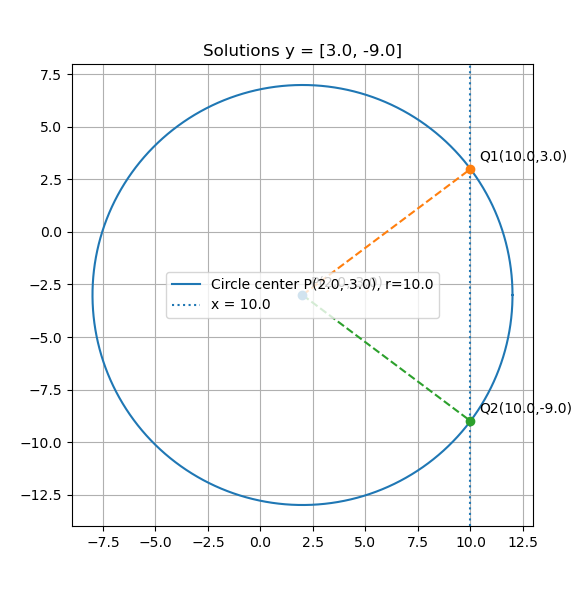
\includegraphics[width=0.6\columnwidth]{figs/fig.png}
\end{center}
\caption{}
\label{fig:Fig1}
\end{figure}
\end{document}
